% This LaTex template is for manuscripts to be included in
% ISCA conference proceedings.
%
\documentclass[letterpaper,twocolumn]{article}
%
\usepackage[raggedright]{titlesec}
%
% include packages as needed, such as
%\usepackage{amsmath}
%\usepackage{amsthm}
\usepackage{graphicx}
%\usepackage[ruled,vlined]{algorithm2e}
%\usepackage{array}
%\usepackage{multirow}
%\usepackage{url}
%\usepackage{subfigure}
%etc.

%no page numbers
\pagestyle{empty}

\setlength{\textwidth}{7.0in}
\setlength{\textheight}{9.125in}
\setlength{\columnsep}{0.375in}
\setlength{\topmargin}{-0.8in}
\setlength{\oddsidemargin}{-0.25in}
\setlength{\evensidemargin}{-0.25in}
\setlength{\parindent}{0.125in}
\setlength{\parskip}{1mm}

\renewcommand\labelenumi{(\theenumi)}

\date{}

\titlespacing{\section}{0pt}{*2.0}{*2.0}
\titlespacing{\subsection}{0pt}{*1.8}{*1.8}

\renewcommand{\topfraction}{0.9}
\renewcommand{\textfraction}{0.1}

\hyphenpenalty=5000
\tolerance=1000

\begin{document}

% Change to your title
\title{\Large\textbf{Lab3 report}\normalsize}

%Chane authors, institutions and emails
\author {Yunxin Sun\\
Department of Computer Science, ETH Zurich\\
Zurich, 8001, Switzerland\\
yunsun@student.ethz.ch
}
\maketitle 

\thispagestyle{empty}

\begin{center}
\large\textbf{Abstract}
\end{center}

\vspace{2mm}
In this lab, we implement two memory scheduling algorithms, BLISS and ATLAS. We then evaluate these two stratigies with four kinds of workloads.
The workload combines both memory-intensive threads and non-memory-intensive threads. Each thread is running alone on one core. 
We evaluate the folllowing metrics for each workload with different stratigies: the instruction throughput and the max slow down. 
The instruction throughput is calculated by the total number of instructions retired devided by totol number of CPU cycles. The max slowdown is calculated by the maximum slowdown of each thread compared with 
running alone on one core. The result shows that ATLAS and BLISS performans almost as equal as traditional 
scheduling algorithms like FRFCFS on four cores, but significantly better(nearly 25\%) on eight cores. 
\medskip
\noindent
% \textbf{keywords:} This part is optional. The word \textbf{keywords} is flushed to the left (no indentation) with 10-point bold font. Include up to 6 keywords. %One space line below the abstract.

\section{Implementation} 
\subsection{ATLAS}
The general idea of ALTAS is to maintain each thread a total attained service and a local attained service.
Since there is only one channel in this lab, we do not consider the synchronization issue. 
After each quantuam, the local service is incorporated into the total service. As one bank can only be occupied 
by one request at one time, we maintain a list of currently serving requests and treat the number of requests belonging to one thread as the number of banks the thread is using.
We maintain this queue by updating information when the channel is also updating the currently serving requests. 
Note here that we put the readiness of the request of top of everything, because it's of no use to schedule a not ready request.
Everything unstated here is exactly the same as in the paper.
\subsection{BLISS} 
The general idea of BLISS is to maintain a blacklist for the thread that is accesing the memory too often and 
get in the way of other threads. We maintain the blacklist in exactly the same way as in the paper. When the memory controller 
continously issues the memory request from the same thread for 4 times, we add that thread into the blacklist. Also note here that, 
in the same way as ATLAS, we put the readiness on top of everything. 

%The sections are just examples. You should make your own sections and sub-sections.

% \section{Related Work}
%
% \section{Methodology}

\section{Results and Analysis}

\subsection{Instruction Throughput Result}
\begin{figure}[!h]
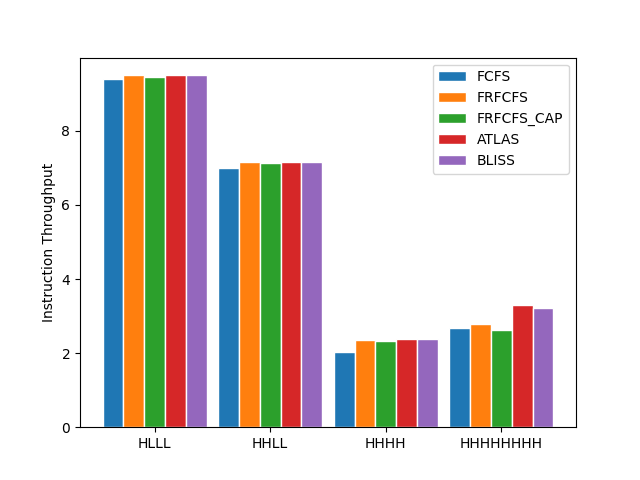
\includegraphics[width=0.4\textwidth]{Figure_1.png}
\end{figure}
This is the result of the instruction throughput of different workload and different scheduling algorithms. 
The ideal instruction throughput should be the number of core multipled by 3(this is the default ipc in Ramulator). However, this is subject to stall and memory access latency, etc. 
One can see that from workload 1 to workload 3, the overall instruction througpuht is smaller 
since more thread is memory-intensive. Workload 4 has an instruction throughput slighly bigger than workload overall. However, considering this is 
an eight-core workload, the situation actually gets worse. One can see that, ALTAS and BLISS performs slightly better in the first three 
workload, but significantly better in the last workload. 
\subsection{Max Slowdown Result}
\begin{figure}[!h]
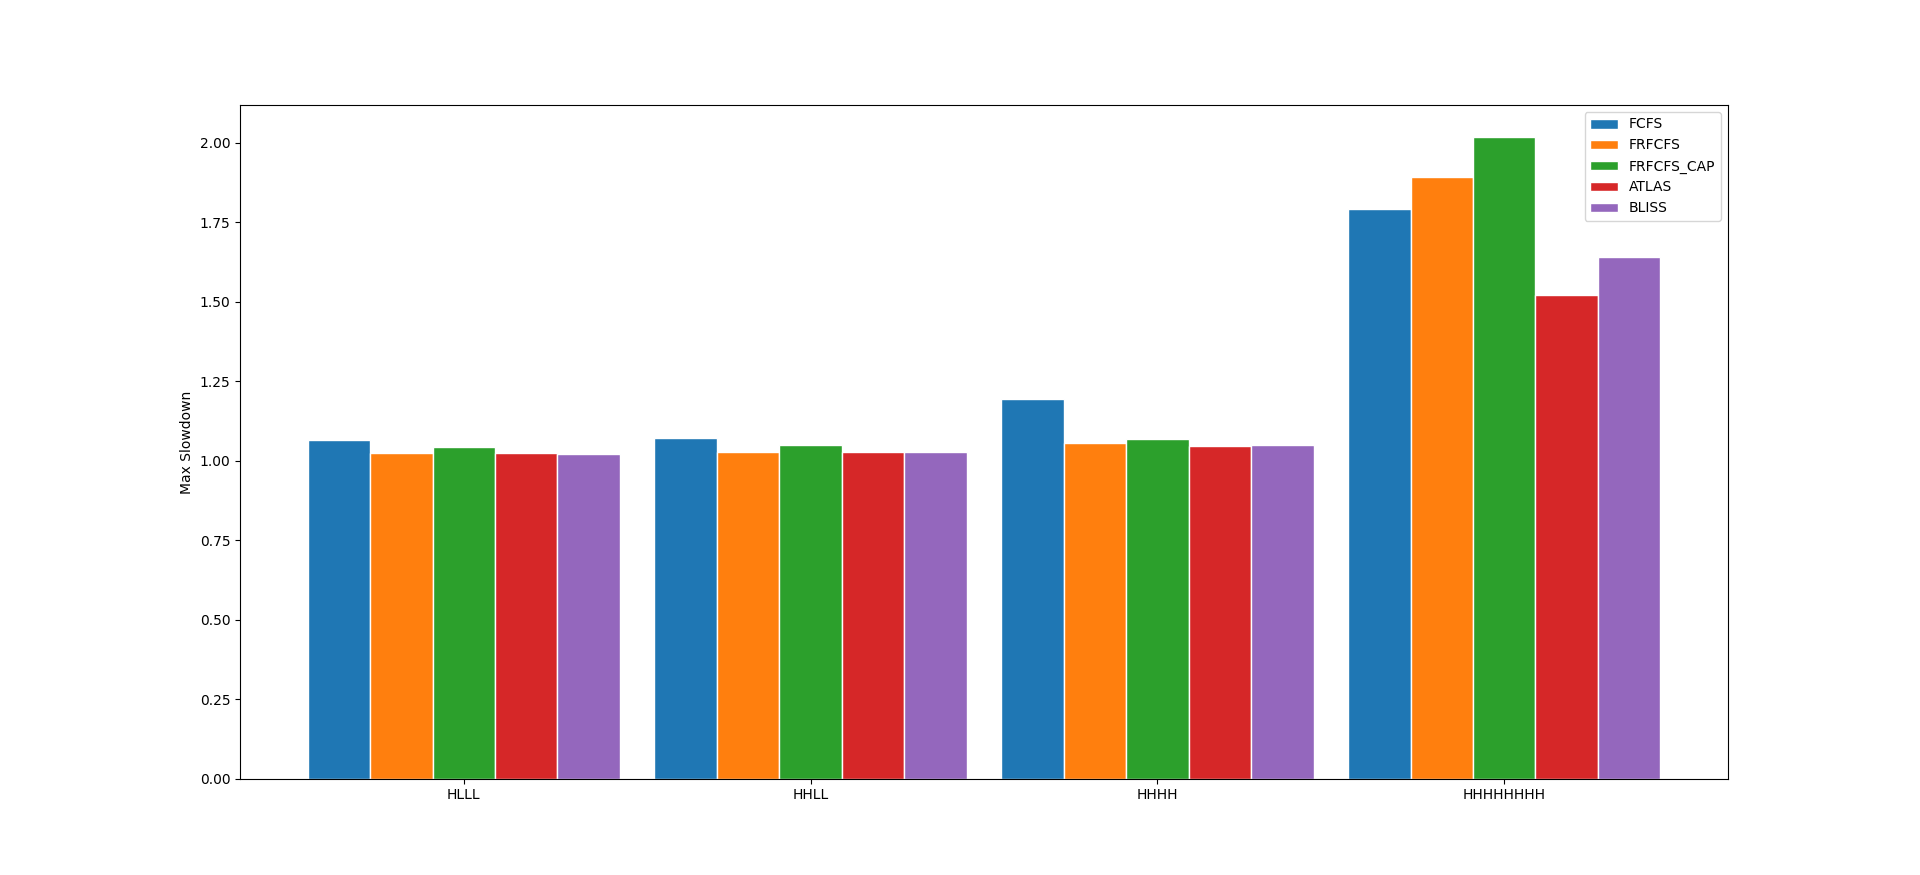
\includegraphics[width=0.4\textwidth]{Figure_2.png}
\end{figure}
This is the result of the max slow down of different workload and different scheduling algorithms. 
One can see that in the first three workload, the max slowdown is only a bit larger than 1, which is desriable(except for the poorest FCFS).
However, in the eight-core setting, the traditional scheduling algorithm(FRFCFS, FCFS, FRFCFS\_CAP) reaches nearly to 2, with the ATLAS and BLISS 
being around 1.5 and 1.6. 
\subsection{Comparision between each policies}
FCFS, FRFCFS and FRFCFS\_CAP does not consider thread level fairnell. I would consider these three 
polices have smaller instruction throughput and larger max slowdown.
% \section{Conclusion}

%You may put all reference items in a separate file, say myRef.bib, in bibTex format.
%
%Here is an example of a myRef.bib file that contains three reference items:
%
%@article{Liben-Nowell-2007,
%author    = {David Liben-Nowell and Jon Kleinberg},
%title     = {The Link Prediction Problem for Social Networks},
%journal   = {Journal of the American Society for Information Science Technology},
%volume    = {58},
%number    = {7},
%year      = {2007},
%pages     = {1019–1031},
%}
%
%@book{Han-2012,
  %author    = {Jiawei Han and Micheline Kamber and Jian Pei},
  %title     = {Data Mining Concepts and Techniques},
  %year      = {2012},
  %edition   = {3rd},
  %publisher = {Morgan Kaufmann}
%}
%
%@inproceedings{Agrawal-1994,
  %author    = {Rakesh Agrawal and Ramakrishnan Srikant},
  %title     = {Fast algorithms for mining association rules},
  %booktitle = {Proceedings of the International Conference on Very Large Databases},
  %year      = {1994},
  %pages     = {487-499},
  %publisher = {ACM Press}
%}
%
%

\bibliographystyle{plain}
\bibliography{myRef} %change to your file name (with suffix .bib)


\end{document} 